
\documentclass[12pt]{article}
\usepackage{graphicx}

\newcommand{\bu}[1] {\textbf{ \underline{#1}}}


\begin{document}

\label{sec:solvent_fit}

\section{SolventFit Instructions}
The SolventFit module is an uncertainty quantification tool for full Bayesian calibration of an Aspen
Plus solvent process model to experimental data. SolventFit
allows for improved predictions with uncertainty bounds by accounting for uncertainty in model parameters
and deficiencies in the model form. The result is a posterior
distribution of parameters allowing for predictions with uncertainty.
The \textbf{\underline{SolventFit}}
algorithm %\citep{Bhat_2015} 
which uses a custom BSS-ANOVA-based response
surface for the outputs. Like the Bayesian inference module, it utilizes Markov Chain Monte Carlo
(MCMC) to compute the posterior distributions, using response surfaces
that serve as fast approximations to the actual simulation model.

To use \textbf{\underline{SolventFit}}, the user will need to install R, as well as the R
packages ``MCMCpack'', ``abind'' and ``MASS''. Please refer to the
installation instructions in Section \ref{(sec.surrogate.acosso)}. 
Once R is installed, the user will also need to set the path to the RScript
executable within FOQUS. 

%%% Insert SolventFit Screenshot

\begin{figure}[h!]
\centering 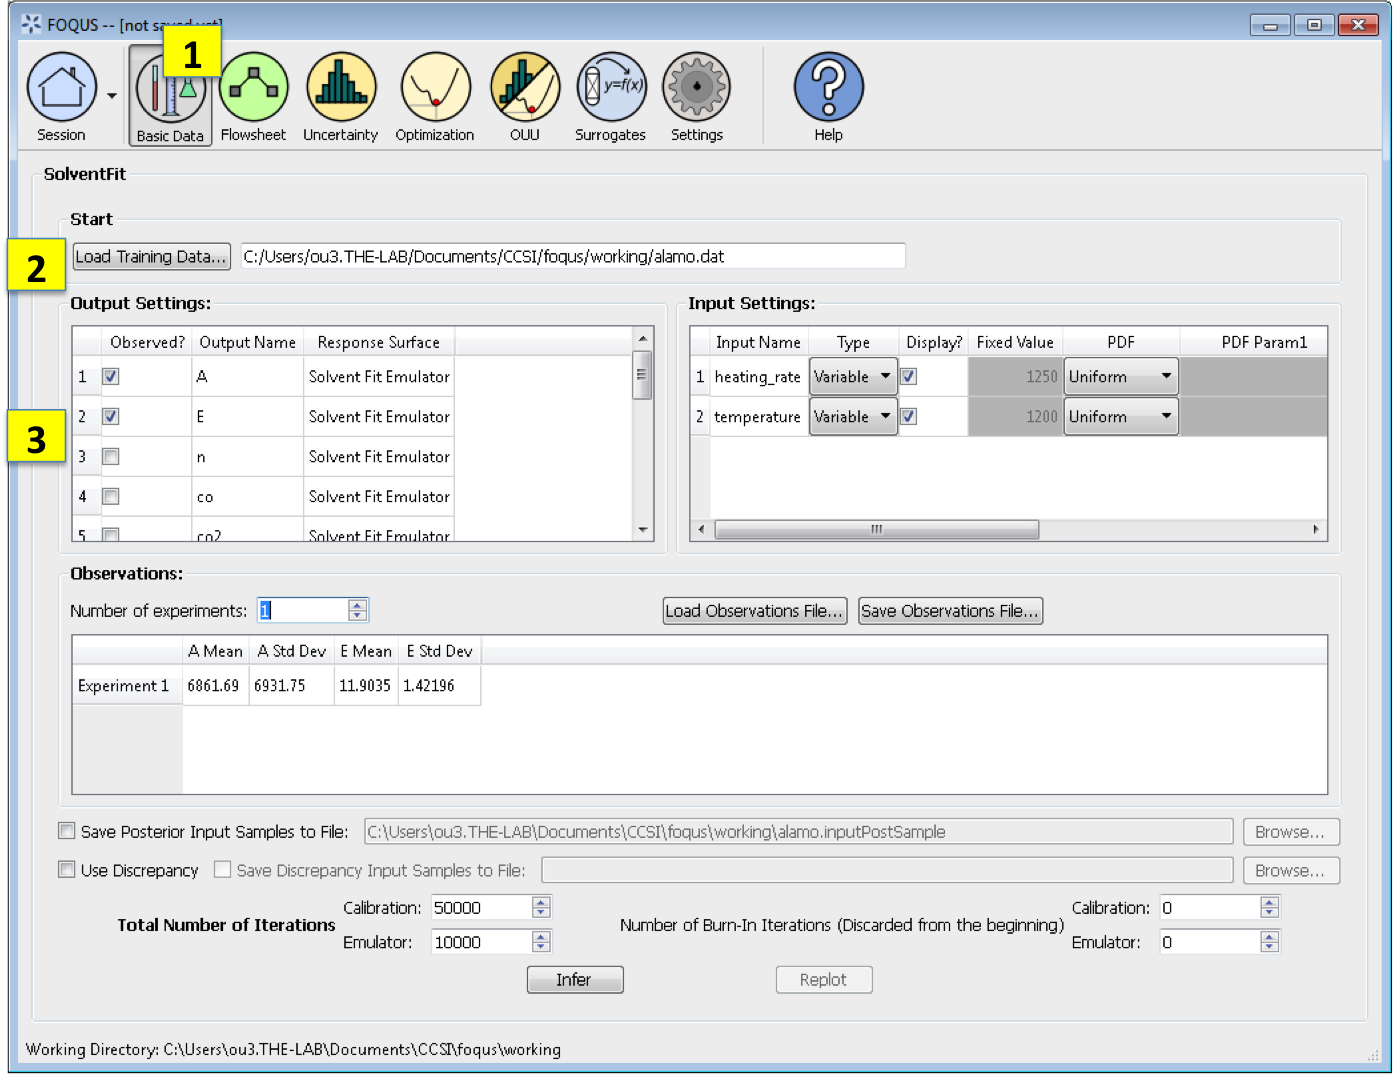
\includegraphics[width=6.5in,height=4in,keepaspectratio]{figs/SolventFitFig1.png}
%\caption{SolventFit Screen}
\label{fig:SolventFit_Fig_1}
\end{figure}

\begin{enumerate}

\item \bu{Basic Data.}  From the FOQUS main screen, click the \bu{Basic Data} button and select \bu{SolventFit} to enter a SolventFit session.

\item \bu{Load Training Data} loads the file of design and variable inputs and their relevant simulation outputs (from Aspen or other computer simulation code).  The file is usually a file with extension .txt, .dat, or .csv.

\item \bu{Output Settings} lists the available outputs for analysis.  The Output Name column lists the name of each output.  The user can select/deselect outputs for analysis using the checkboxes in the Observed column.  The response surface in SolventFit will be prepopulated with ``SolventFit Emulator'' because SolventFit uses its own custom BSS-ANOVA response surface model.  The simulation ensemble is used as the training data for generating the response surfaces.

\begin{figure}[h!]
\centering 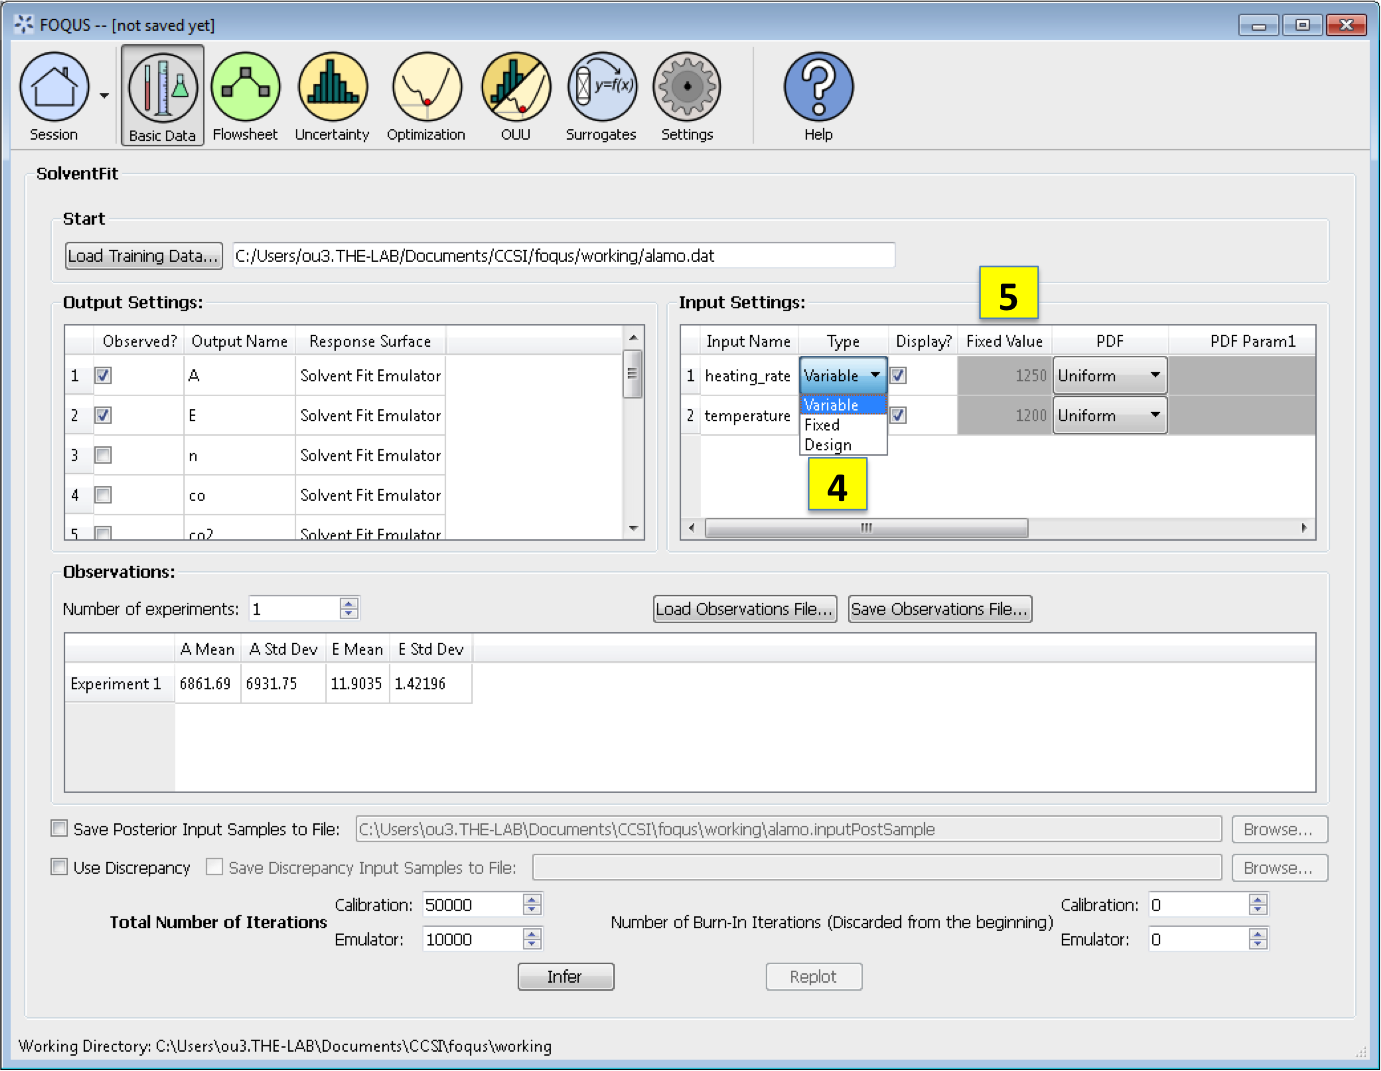
\includegraphics[width=6.5in,height=4in,keepaspectratio]{figs/SolventFitFig2.png}
%\caption{Bayesian Inference Dialog}
\label{fig:SolventFit_Fig_2}
\end{figure}

\item  \bu{Input Settings} is populated with input variable information from the training data.  Under the column, \bu{Type}, user can specify which inputs are fixed, design, or variable using the from the drop-down menu in the \bu{Input Settings Table}.  Selecting ``Fixed" means that the input is fixed at its default value for all design points. Changing the type to ``Variable" means that the input is a calibration parameter and is uncertain; therefore, its value varies between samples.   Changing the type to ``Design" means that the input is an experimental inputs with preselected values, and are also inputs in the experimental data.  In addition, the user can specify which inputs are displayed in the resulting plots of the posterior distributions.  To omit specific inputs, clear the checkboxes from the \textbf{\underline{Display}} column of the table.  (By default, once inference completes, all inputs will be
displayed in the plots.)   

\item \bu{Fixed Value.} With any fixed input, the only parameter that can be changed is the default value (i.e., all samples of this input are fixed at this default value). 

\begin{figure}[h!]
\centering \includegraphics[width=6.5in,height=4in,keepaspectratio]{figs/SolventFitFig3.png}
%\caption{Bayesian Inference Dialog}
\label{fig:SolventFit_Fig_3}
\end{figure}

\item \bu{PDF.} With any variable input, the minimum/maximum values, as well as the probability distribution function (PDF), for that input can be changed.  The default prior is specified to be Uniform.   To change the prior distribution type (e.g.,  Uniform, Normal, Lognormal, or Gamma), use the drop-down list in the \textbf{\underline{PDF}} column (box 6a) and enter corresponding values for the PDF parameters. To change the range of a uniform prior, scroll all the way to the right to modify \textbf{\underline{Min/Max}}. 

\begin{figure}[h!]
\centering 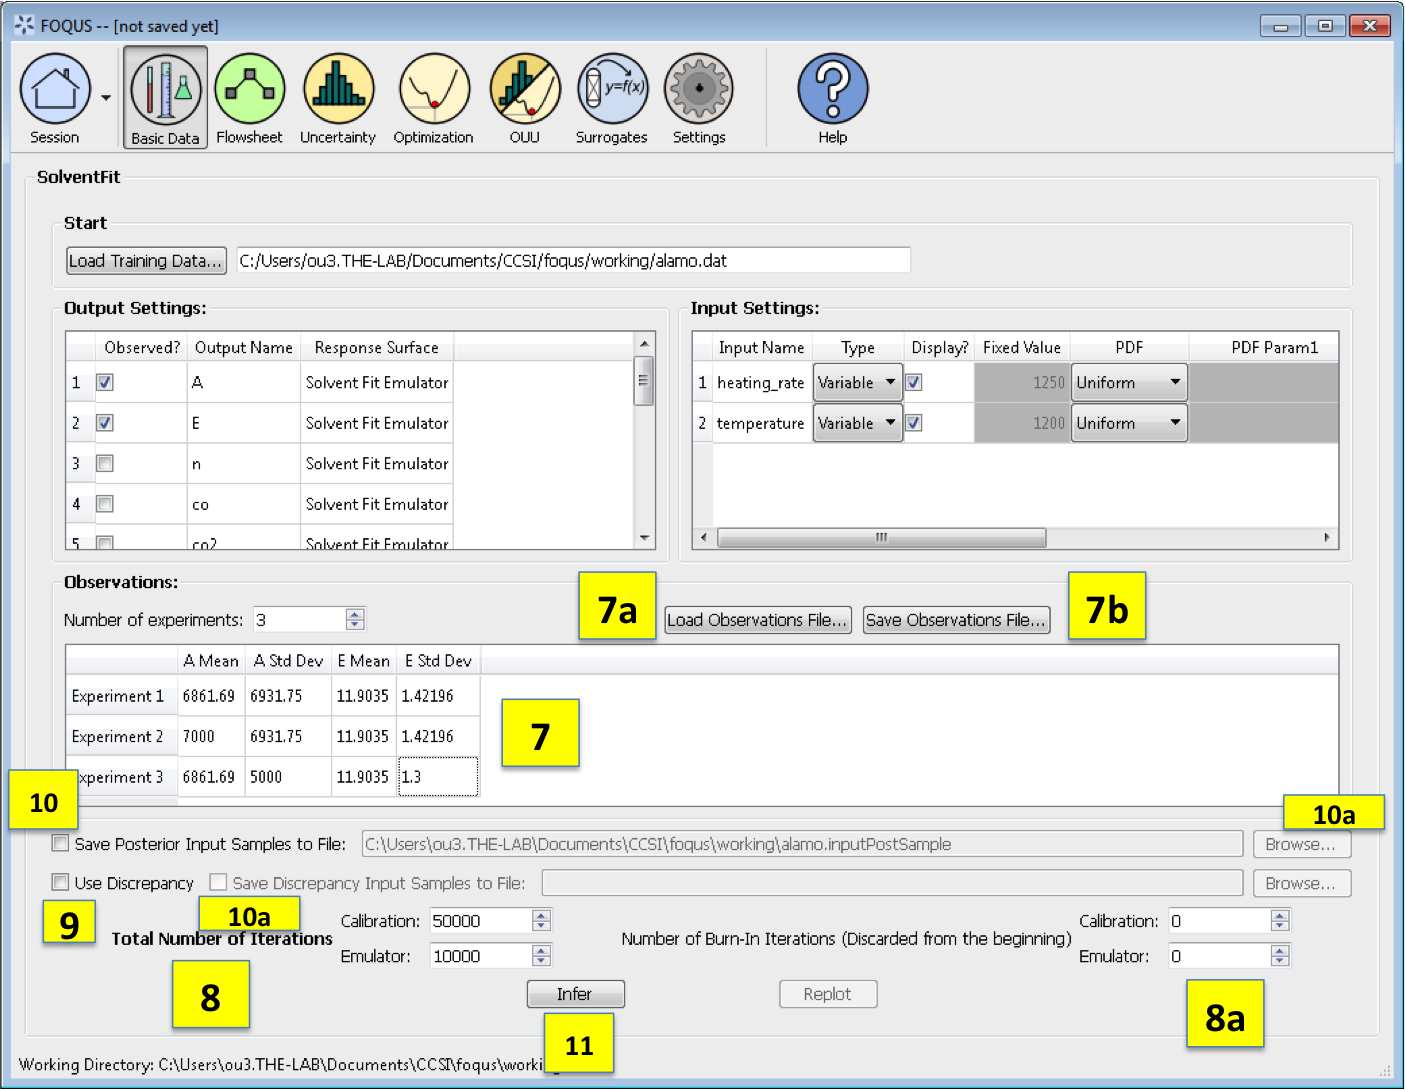
\includegraphics[width=6.5in,height=4in,keepaspectratio]{figs/SolventFitFig4.png}
%\caption{Bayesian Inference Dialog}
\label{fig:SolventFit_Fig_4}
\end{figure}

\item \bu{Observations} section enables the user to add experimental data in the form of observations of certain output variables.
   At least one observation is required; the \bu{number of experiments} may be changed using the pull down menu.  For each observation, enter the mean and standard deviation (enter zero if there is no information about the noise) for all of the outputs.  If any inputs are selected as design inputs, their values will also be required here.  Currently, the observation noise model is assumed to be a normal distribution.  
Alternatively, the user can import the file of experiments using the \bu{Load Observation File} button (7a).  The user can also export the observations using the \bu{Save Observation File} button (7b).    

\item \bu{Number of Iterations} are the number of iterations that the Markov Chain Monte Carlo (MCMC) is run for emulation and calibration.  The default is set at 10000 for emulation and 50000 for calibration.  Also the number of ``burn-in" samples (number of initial samples to be thrown out) for both emulation and calibration may be changed from its default of 0 using the relevant button (8a).   

\item \bu{Use Discrepancy.}  Check this box if the discrepancy should be estimated in the calibration model.  It is usually good practice to include the discrepancy.

\item \bu{Save Posterior Input Samples to File} checkbox, when selected, saves the posterior input samples as a PSUADE sample file (format described in Section \ref{ap:psuadefiles}). This file characterizes the input uncertainty as a set of samples, %which can be re-used in the \textbf{\underline{Simulation EnsembleSetup}} dialog, to evaluate the outputs corresponding to these posterior input samples.  
In addition, the user can save the discrepancy samples to a file by selecting the checkbox \bu{Save Discrepancy Input Samples to File} (10a).  If saving posterior and/or discrepancy samples to a file, click \bu{Browse} to set the name and location of where this file is saved (10b).

\item Click \bu{Infer} to start the analysis. (Note: If the inference returns an invalid posterior distribution (i.e., one with no samples), it
	usually means the prior distributions or that the observation data distributions are not prescribed appropriately. In this case, it is
	recommended that the user experiment with different priors and/or data distribution means and/or standard deviations.)
	
\item The plotted results for SolventFit are posterior distributions of the selected variable inputs which are similar to the plots from the Bayesian Inference in the Uncertainty Quantification module, see the section on Bayesian Inference for more details.  	




%\item{Inference calculations often take a very long time. If inference has
%	run to completion, use \bu{Replot} to generate new plots (e.g., to only
%	display a subset of the input posterior graphs) from the cached
%	inference results.}


\end{enumerate}



\end{document}